\documentclass[a4paper,12pt]{article}

\usepackage[a4paper,margin=1in]{geometry}
\usepackage{amsmath,amssymb,bm}
\usepackage{array}
\usepackage{algorithm}
\usepackage{algpseudocode}
\usepackage{booktabs}
\usepackage{caption}
\usepackage{enumitem}
\usepackage{fancyhdr}
\usepackage{float}
\usepackage{graphicx}
\usepackage[colorlinks=true,linkcolor=blue!60!black,citecolor=green!40!black,urlcolor=blue!60!black]{hyperref}
\usepackage{subcaption}
\usepackage{tabularx}
\usepackage{tikz}
\usetikzlibrary{arrows.meta,calc,fit,positioning,shapes.geometric}
\usepackage[table]{xcolor}

\setlength{\parindent}{0pt}
\setlength{\parskip}{0.65em}
\setlength{\headheight}{15pt}
\renewcommand{\arraystretch}{1.2}
\graphicspath{{report_assets/}}

% Color palette adapted from the slide deck to keep visual continuity.
\definecolor{BgBase}{HTML}{F6F8FF}
\definecolor{BgSurface}{HTML}{E6ECFF}
\definecolor{BgElevated}{HTML}{CDD6FF}
\definecolor{TextPrimary}{HTML}{111827}
\definecolor{TextMuted}{HTML}{4B5563}
\definecolor{AccentMain}{HTML}{3D52CC}
\definecolor{AccentSoft}{HTML}{C7CFFF}
\definecolor{Highlight}{HTML}{BE185D}
\definecolor{HighlightSoft}{HTML}{FBCFE8}

\hypersetup{
    pdftitle={Diffusion Models Report},
    pdfauthor={Anindya Biswas, Tasnim Tamal, Din Mohammad},
}

\pagestyle{fancy}
\fancyhf{}
\fancyhead[L]{CSE 200}
\fancyhead[R]{Diffusion Models}
\fancyfoot[C]{\thepage}

\newcommand{\vect}[1]{\bm{#1}}
\newcommand{\E}{\mathbb{E}}
\newcommand{\R}{\mathbb{R}}
\newcommand{\alphabar}{\bar{\alpha}}
\newcommand{\reporttitle}{Diffusion Models}

\begin{document}

\hypersetup{pageanchor=false}
\begin{titlepage}

\begin{tikzpicture}[remember picture,overlay]
    \fill[HighlightSoft,opacity=0.45] ([xshift=-1.6cm,yshift=1.4cm]current page.north east) circle (4.7cm);
    \fill[AccentSoft,opacity=0.55] ([xshift=1.2cm,yshift=-1.0cm]current page.south west) circle (4.4cm);
    \fill[BgElevated,opacity=0.85] ([xshift=-0.6cm,yshift=0.8cm]current page.north east) circle (2.0cm);
\end{tikzpicture}

\centering
\vspace*{1.3cm}

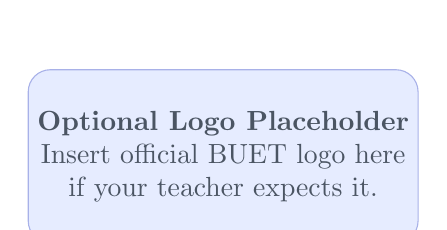
\begin{tikzpicture}
    \node[
        draw=AccentMain!45,
        fill=BgSurface,
        rounded corners=8pt,
        minimum width=4.4cm,
        minimum height=2.2cm,
        align=center,
        text=TextMuted
    ] {\textbf{Optional Logo Placeholder}\\Insert official BUET logo here\\if your teacher expects it.};
\end{tikzpicture}

\vspace{0.8cm}
{\Large\textbf{Bangladesh University of Engineering and Technology}}\\[0.2cm]
{\large Department of Computer Science and Engineering}\\[0.2cm]
{\large CSE 200 -- Technical Writing and Presentation}\\[1.3cm]

{\Huge\bfseries\color{AccentMain}\reporttitle}\\[0.3cm]
{\Large How AI Learns to Generate Images from Noise}\\[0.5cm]
\rule{0.85\linewidth}{0.8pt}\\[0.8cm]

\begin{minipage}{0.82\linewidth}
\centering
\textbf{Prepared from our presentation slides on diffusion models and expanded into a formal technical report.}
\end{minipage}

\vfill

\begin{tabular}{>{\bfseries}p{3.0cm}p{8.3cm}}
Submitted by & Anindya Biswas \dotfill Student ID: 2205107 \\
             & Tasnim Tamal \dotfill Student ID: 2205110 \\
             & Din Mohammad \dotfill Student ID: 2205113 \\
\addlinespace
Date & \today \\
\end{tabular}

\vfill
{\large\color{TextMuted}Report prepared in \LaTeX{} with original TikZ diagrams and locally available slide assets.}
\end{titlepage}
\hypersetup{pageanchor=true}

\pagenumbering{roman}
\tableofcontents
\listoffigures
\listoftables
\newpage
\pagenumbering{arabic}

\section*{Abstract}
Diffusion models are a family of generative models that synthesize realistic data by learning how to reverse a gradual noising process. Instead of producing an image in a single step, the model starts from random noise and iteratively removes corruption until a structured sample appears. This report expands the material presented in our slide deck into a formal written explanation. It introduces the motivation behind modern generative modeling, explains the forward and reverse diffusion processes, summarizes the role of the U-Net backbone and timestep conditioning, and presents the standard noise-prediction objective used in Denoising Diffusion Probabilistic Models (DDPMs) \cite{ho2020ddpm,nichol2021improved}. The report also highlights why diffusion models are attractive in practice: they train more stably than many adversarial methods, produce high-quality samples, and support conditional generation for images, video, and scientific design \cite{song2019generative,rombach2022latent}. Finally, their main limitations are discussed, including slow sampling, large computational cost, and the need for responsible deployment. Throughout the report, the emphasis is on clear technical writing, interpretable diagrams, and consistent visual presentation.

\section{Introduction}
Generative modeling asks a simple but ambitious question: can a machine learn the underlying distribution of real data well enough to create new samples that appear authentic? In the context of images, this means producing outputs that preserve global structure, local texture, and semantic coherence. Recent diffusion-based approaches have become a major answer to this problem because they combine principled probabilistic modeling with impressive empirical performance \cite{ho2020ddpm,song2020ddim}.

Figure~\ref{fig:motivation-real-vs-ai} illustrates the motivation behind the topic. To a human observer, the image on the right can look plausible even though it is generated by a model. The challenge for a generative model is therefore not only to memorize training examples, but to learn a rich data distribution from which new samples can be drawn.

\begin{figure}[H]
    \centering
    \begin{subfigure}[b]{0.38\linewidth}
        \centering
        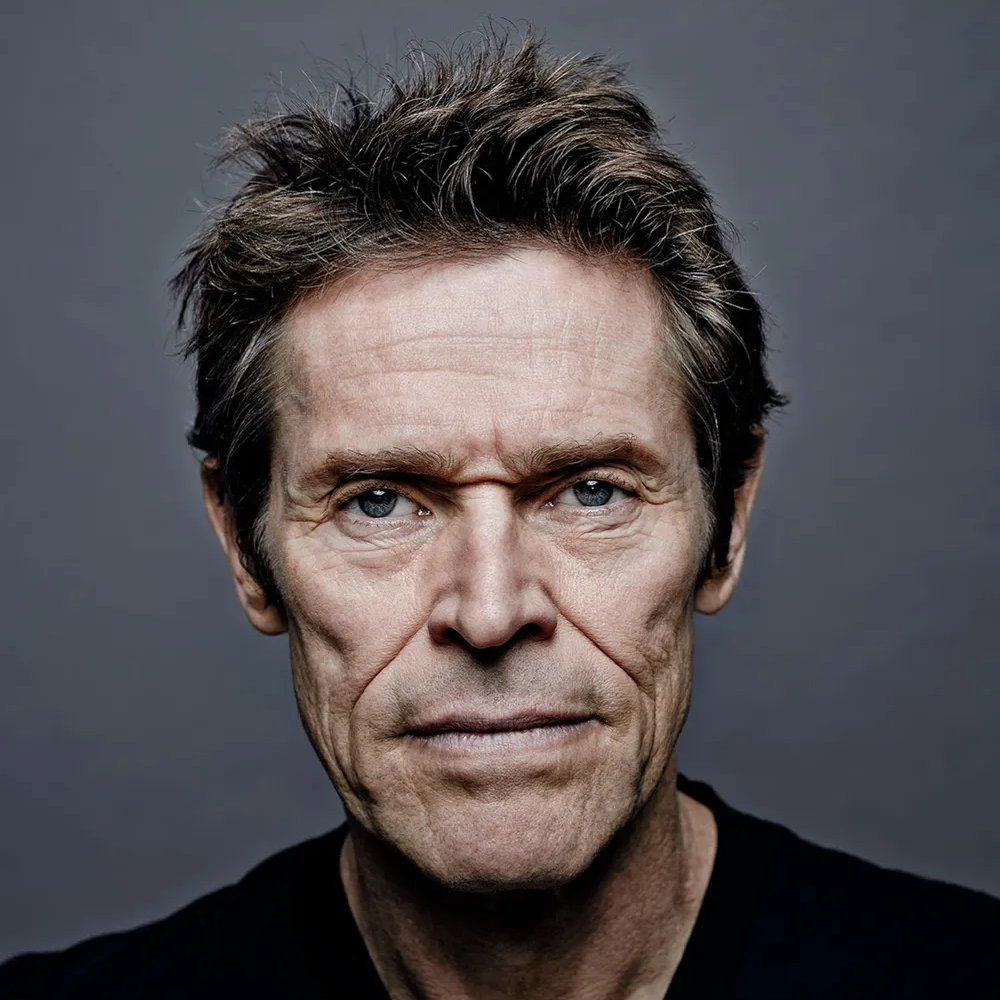
\includegraphics[width=\linewidth]{real_face.png}
        \caption{A real face sample.}
    \end{subfigure}
    \hfill
    \begin{subfigure}[b]{0.38\linewidth}
        \centering
        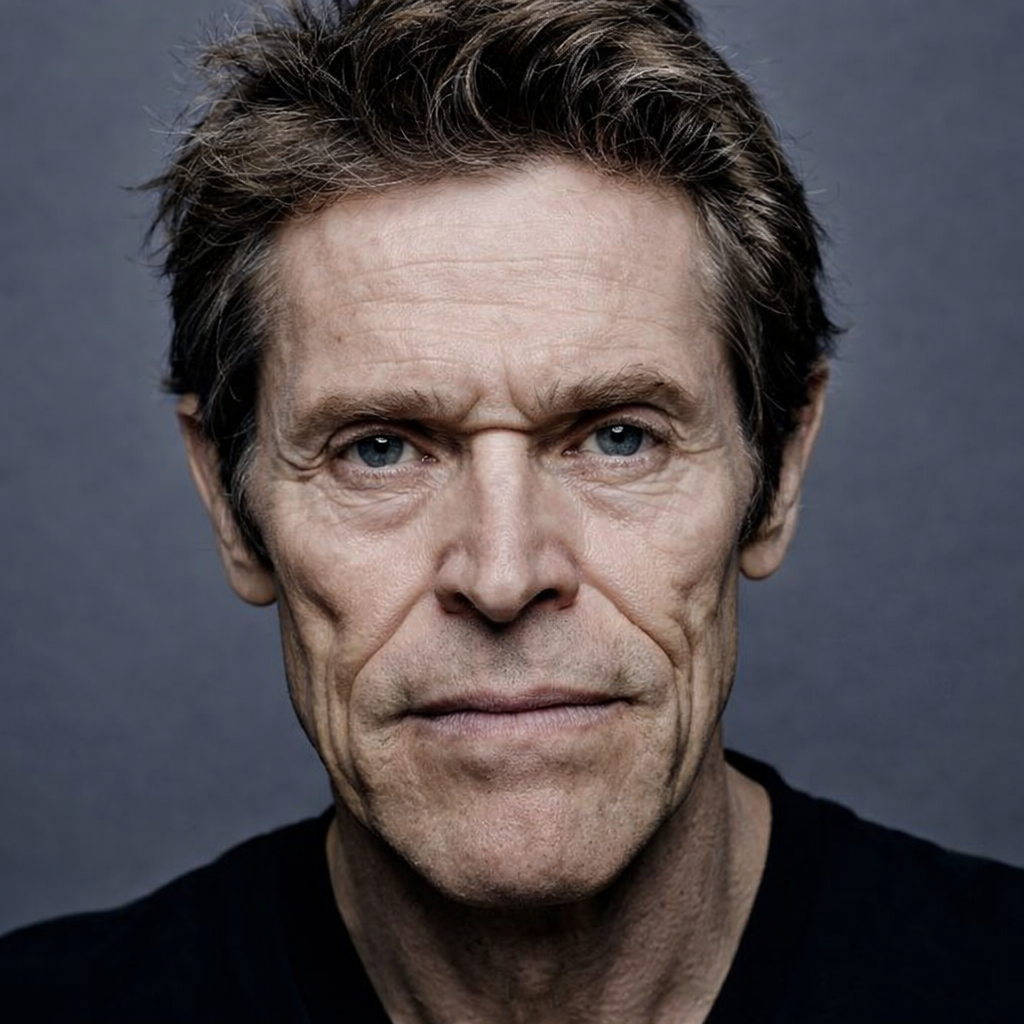
\includegraphics[width=\linewidth]{ai_face.png}
        \caption{A model-generated face sample.}
    \end{subfigure}
    \caption{A motivating comparison between real data and synthetic data. Diffusion models aim to generate samples that are visually consistent with the underlying real-data distribution.}
    \label{fig:motivation-real-vs-ai}
\end{figure}

The key idea behind diffusion models is surprisingly intuitive. During training, the model sees real data that is gradually corrupted with small amounts of Gaussian noise. Because the corruption process is controlled mathematically, the model can then be trained to predict the noise that was added. At generation time, the procedure is reversed: the model begins with pure noise and denoises it step by step until a realistic sample emerges. This decomposition turns a difficult generative task into a sequence of simpler prediction steps.

\section{Core Diffusion Mechanism}
The workflow of a diffusion model has two complementary parts: a \textit{forward diffusion process} that destroys information and a \textit{reverse diffusion process} that reconstructs structure. Figure~\ref{fig:diffusion-overview} summarizes this idea in one diagram.

\begin{figure}[H]
    \centering
    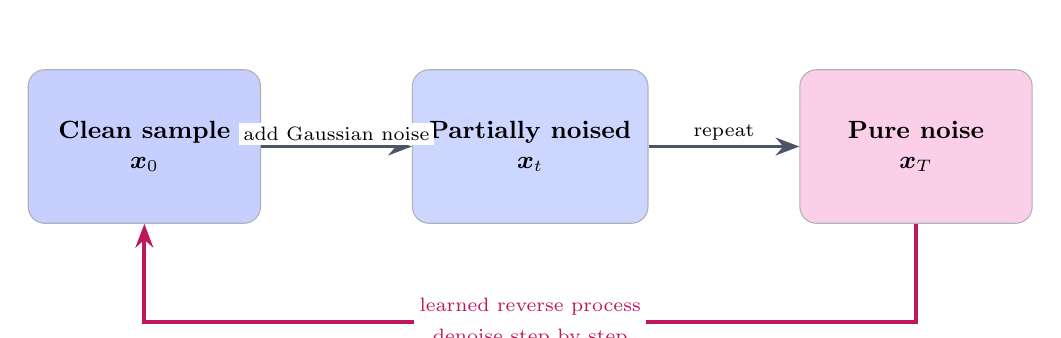
\begin{tikzpicture}[
        font=\small,
        stage/.style={
            rounded corners=6pt,
            draw=TextMuted!45,
            minimum width=2.95cm,
            minimum height=1.95cm,
            align=center,
            inner sep=6pt
        },
        farr/.style={-{Stealth[length=3mm]}, line width=1.3pt, draw=TextMuted},
        rarr/.style={-{Stealth[length=3mm]}, line width=1.5pt, draw=Highlight}
    ]
        \node[stage, fill=AccentSoft] (x0) at (0,0) {\textbf{Clean sample}\\$\vect{x}_0$};
        \node[stage, fill=BgElevated] (xt) at (4.9,0) {\textbf{Partially noised}\\$\vect{x}_t$};
        \node[stage, fill=HighlightSoft] (xT) at (9.8,0) {\textbf{Pure noise}\\$\vect{x}_T$};

        \draw[farr] (x0) -- (xt)
            node[midway, above, fill=white, inner sep=1.5pt] {\scriptsize add Gaussian noise};
        \draw[farr] (xt) -- (xT)
            node[midway, above, fill=white, inner sep=1.5pt] {\scriptsize repeat};

        \coordinate (revmid) at ($(xt.south)+(0,-1.25)$);
        \draw[rarr] (xT.south) |- (revmid) -| (x0.south);
        \node[text=Highlight, align=center, fill=white, inner sep=2pt] at (revmid)
            {\scriptsize learned reverse process\\\scriptsize denoise step by step};
    \end{tikzpicture}
    \caption{Conceptual overview of diffusion models. Training uses the controlled noising path, while sampling uses the learned reverse path.}
    \label{fig:diffusion-overview}
\end{figure}

\subsection{Forward Diffusion}
The forward process is a Markov chain that progressively perturbs a clean sample $\vect{x}_0 \in \R^d$ with Gaussian noise. At each timestep $t$, a small variance term $\beta_t$ determines how much corruption is introduced:
\begin{equation}
    q(\vect{x}_t \mid \vect{x}_{t-1}) =
    \mathcal{N}\!\left(\sqrt{1-\beta_t}\,\vect{x}_{t-1}, \beta_t \vect{I}\right).
    \label{eq:forward-markov}
\end{equation}

If we define $\alpha_t = 1-\beta_t$ and $\alphabar_t = \prod_{s=1}^{t}\alpha_s$, then a sample at any timestep can be written directly as
\begin{equation}
    \vect{x}_t = \sqrt{\alphabar_t}\,\vect{x}_0 + \sqrt{1-\alphabar_t}\,\vect{\epsilon},
    \quad \vect{\epsilon} \sim \mathcal{N}(\vect{0}, \vect{I}).
    \label{eq:closed-form-forward}
\end{equation}

Equation~\ref{eq:closed-form-forward} is especially useful during training because it allows the model to jump directly to a randomly chosen timestep without simulating every previous step.

\begin{figure}[H]
    \centering
    \begin{subfigure}[b]{0.22\linewidth}
        \centering
        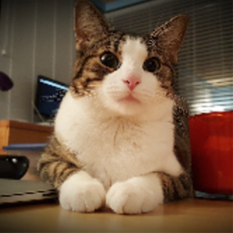
\includegraphics[width=\linewidth]{clean.png}
        \caption{Clean}
    \end{subfigure}
    \hfill
    \begin{subfigure}[b]{0.22\linewidth}
        \centering
        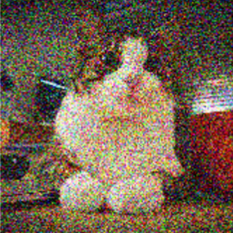
\includegraphics[width=\linewidth]{noised_slightly.png}
        \caption{Low noise}
    \end{subfigure}
    \hfill
    \begin{subfigure}[b]{0.22\linewidth}
        \centering
        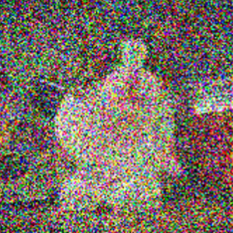
\includegraphics[width=\linewidth]{noised_heavily.png}
        \caption{Heavy noise}
    \end{subfigure}
    \hfill
    \begin{subfigure}[b]{0.22\linewidth}
        \centering
        
\includegraphics[width=\linewidth]{noised_fully.png}
        \caption{Pure noise}
    \end{subfigure}
    \caption{Visual interpretation of the forward diffusion process. A structured image is gradually transformed into an approximately Gaussian sample.}
    \label{fig:progressive-noising}
\end{figure}

\subsection{Reverse Diffusion}
Once the data has been corrupted, the generative task becomes the reverse problem: infer how to move from $\vect{x}_t$ back to a less noisy sample $\vect{x}_{t-1}$. The model parameterized by $\theta$ learns a reverse distribution of the form
\begin{equation}
    p_{\theta}(\vect{x}_{t-1} \mid \vect{x}_t) =
    \mathcal{N}\!\left(\vect{\mu}_{\theta}(\vect{x}_t,t), \vect{\Sigma}_{\theta}(\vect{x}_t,t)\right).
    \label{eq:reverse-process}
\end{equation}

In practice, many popular implementations train a neural network to predict the added noise rather than predicting pixels directly. This reparameterization makes learning easier because the model only needs to estimate the perturbation that separates $\vect{x}_t$ from the underlying clean sample \cite{ho2020ddpm,nichol2021improved}.

\section{Model Architecture and Training}
The success of a diffusion model depends not only on the probabilistic formulation, but also on a strong neural architecture. Most image diffusion systems use a U-Net-like backbone with multi-scale feature extraction and skip connections \cite{ronneberger2015unet}. The network receives two inputs: a noisy image $\vect{x}_t$ and an embedding of the timestep $t$.

\begin{figure}[H]
    \centering
    \resizebox{0.97\linewidth}{!}{%
    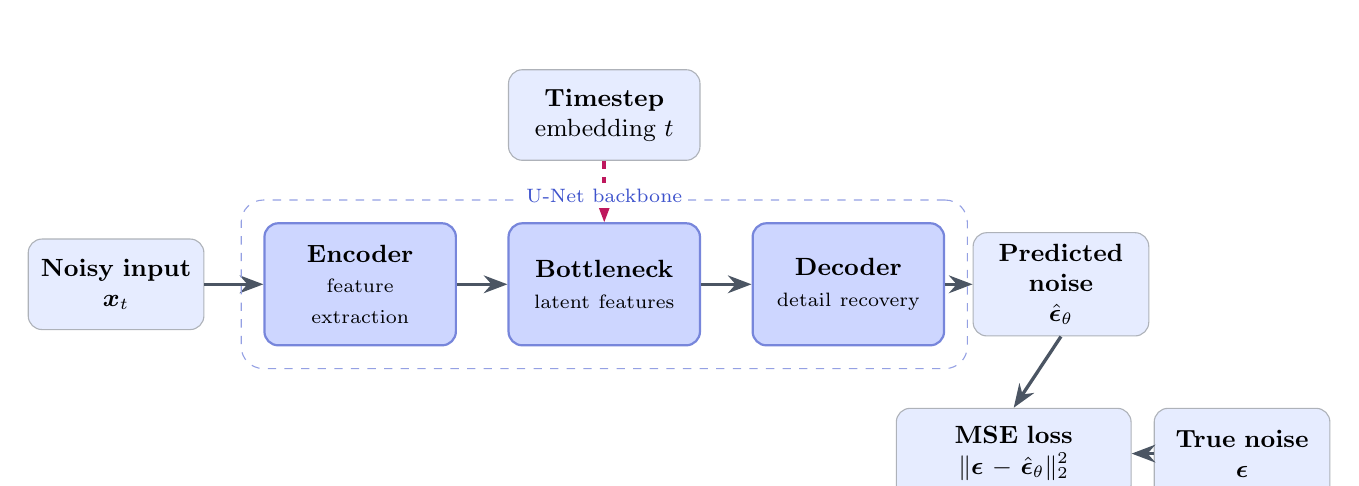
\begin{tikzpicture}[
        font=\small,
        box/.style={
            rounded corners=5pt,
            draw=AccentMain!70,
            fill=BgElevated,
            thick,
            text width=2.15cm,
            minimum height=1.55cm,
            align=center,
            inner sep=4pt
        },
        softbox/.style={
            rounded corners=5pt,
            draw=TextMuted!45,
            fill=BgSurface,
            text width=1.95cm,
            minimum height=1.15cm,
            align=center,
            inner sep=4pt
        },
        arrow/.style={-{Stealth[length=3mm]}, line width=1.2pt, draw=TextMuted},
        hiarrow/.style={-{Stealth[length=3mm]}, line width=1.3pt, draw=Highlight}
    ]
        \node[softbox] (input) at (0,0) {\textbf{Noisy input}\\$\vect{x}_t$};
        \node[box] (enc) at (3.1,0) {\textbf{Encoder}\\\scriptsize feature extraction};
        \node[box] (bottleneck) at (6.2,0) {\textbf{Bottleneck}\\\scriptsize latent features};
        \node[box] (dec) at (9.3,0) {\textbf{Decoder}\\\scriptsize detail recovery};
        \node[softbox] (epshat) at (12.0,0) {\textbf{Predicted noise}\\$\hat{\vect{\epsilon}}_{\theta}$};

        \node[softbox, text width=2.15cm] (time) at (6.2,2.15) {\textbf{Timestep}\\embedding $t$};
        \node[softbox, text width=2.7cm] (loss) at (11.4,-2.15) {\textbf{MSE loss}\\$\|\vect{\epsilon}-\hat{\vect{\epsilon}}_{\theta}\|_2^2$};
        \node[softbox, text width=1.95cm] (epstrue) at (14.3,-2.15) {\textbf{True noise}\\$\vect{\epsilon}$};

        \draw[arrow] (input) -- (enc);
        \draw[arrow] (enc) -- (bottleneck);
        \draw[arrow] (bottleneck) -- (dec);
        \draw[arrow] (dec) -- (epshat);
        \draw[hiarrow, dashed] (time) -- (bottleneck);
        \draw[arrow] (epshat.south) -- (loss.north);
        \draw[arrow] (epstrue.west) -- (loss.east);

        \node[
            draw=AccentMain!55,
            dashed,
            rounded corners=8pt,
            inner sep=8pt,
            fit=(enc)(bottleneck)(dec)
        ] (unetfit) {};
        \node[text=AccentMain, fill=white, inner sep=2pt] at ($(unetfit.north)+(0,0.05)$) {\scriptsize U-Net backbone};
    \end{tikzpicture}%
    }
    \caption{A simplified training view of an image diffusion model. The network receives a noisy image and the current timestep, predicts the noise component, and is trained with a mean-squared error objective.}
    \label{fig:unet-training}
\end{figure}

\subsection{Noise-Prediction Objective}
The standard DDPM training objective is
\begin{equation}
    \mathcal{L}_{\text{simple}}
    =
    \E_{\vect{x}_0,t,\vect{\epsilon}}
    \left[
        \left\|
            \vect{\epsilon} - \vect{\epsilon}_{\theta}(\vect{x}_t,t)
        \right\|_2^2
    \right].
    \label{eq:noise-objective}
\end{equation}

This loss is attractive because the target noise $\vect{\epsilon}$ is known exactly; it was sampled by the training procedure itself. As a result, the model is optimized with a clean and well-defined supervision signal. Compared with directly generating pixels in one shot, this approach decomposes a hard problem into many small denoising tasks.

\subsection{Training Workflow}
The complete training routine can be summarized as Algorithm~\ref{alg:diffusion-training}. The procedure alternates between sampling a real image, corrupting it to a random timestep, and updating the network so that its predicted noise matches the actual perturbation.

\begin{algorithm}[H]
\caption{Training a diffusion model with noise prediction}
\label{alg:diffusion-training}
\begin{algorithmic}[1]
\Require Training dataset $\mathcal{D}$, noise schedule $\{\beta_t\}_{t=1}^{T}$, neural network $\vect{\epsilon}_{\theta}$
\While{training has not converged}
    \State Sample a clean image $\vect{x}_0 \sim \mathcal{D}$
    \State Sample a timestep $t$ uniformly from $\{1,\dots,T\}$
    \State Sample Gaussian noise $\vect{\epsilon} \sim \mathcal{N}(\vect{0},\vect{I})$
    \State Form a noisy input using Equation~\ref{eq:closed-form-forward}
    \State Predict $\hat{\vect{\epsilon}} = \vect{\epsilon}_{\theta}(\vect{x}_t,t)$
    \State Compute $\mathcal{L}_{\text{simple}} = \|\vect{\epsilon} - \hat{\vect{\epsilon}}\|_2^2$
    \State Update $\theta$ using gradient descent
\EndWhile
\end{algorithmic}
\end{algorithm}

Table~\ref{tab:notation} collects the most important symbols used in the mathematical discussion so that the notation remains easy to follow.

\begin{table}[H]
    \centering
    \begin{tabularx}{\linewidth}{>{\bfseries}p{2.2cm}X}
        \toprule
        Symbol & Meaning \\
        \midrule
        $\vect{x}_0$ & A clean training sample drawn from the data distribution. \\
        $\vect{x}_t$ & The noisy version of the sample at diffusion step $t$. \\
        $\beta_t$ & Variance schedule controlling how much noise is added at step $t$. \\
        $\alpha_t$ & Shorthand for $1-\beta_t$. \\
        $\alphabar_t$ & Cumulative product $\prod_{s=1}^{t}\alpha_s$, measuring the remaining signal after $t$ steps. \\
        $\vect{\epsilon}$ & Gaussian noise used to corrupt the sample. \\
        $\vect{\epsilon}_{\theta}(\vect{x}_t,t)$ & Neural network prediction of the added noise. \\
        \bottomrule
    \end{tabularx}
    \caption{Notation used in the forward process, reverse process, and training objective.}
    \label{tab:notation}
\end{table}

\section{Why Diffusion Models Work Well}
The practical success of diffusion models comes from a balance of theory and engineering. First, the model is trained on a supervised target that is generated directly by the noising process. This makes optimization comparatively stable. Second, the model denoises iteratively, so global structure and local texture can emerge gradually rather than being forced into a single network output. Third, conditioning information such as text, class labels, or masks can be injected naturally into the denoising network.

These properties help explain why diffusion systems became competitive with, and in many settings superior to, earlier generative approaches. Table~\ref{tab:model-comparison} gives a concise comparison that highlights typical trade-offs.

\begin{table}[H]
    \centering
    \rowcolors{2}{BgBase}{white}
    {\small
    \begin{tabularx}{\linewidth}{>{\raggedright\arraybackslash\bfseries}p{1.95cm}>{\raggedright\arraybackslash}p{2.15cm}>{\raggedright\arraybackslash}p{1.85cm}>{\raggedright\arraybackslash}p{1.8cm}>{\raggedright\arraybackslash}X}
        \toprule
        \shortstack[l]{Model\\family} &
        \shortstack[l]{Training\\stability} &
        \shortstack[l]{Sample\\quality} &
        \shortstack[l]{Sampling\\speed} &
        Main comment \\
        \midrule
        VAE & High & Moderate & Fast & Strong probabilistic interpretation but often blurrier outputs. \\
        GAN & Moderate to low & High & Very fast & Can generate sharp images but training may be unstable and prone to mode collapse. \\
        Diffusion model & High & Very high & Slow & Excellent fidelity and diversity, but generation requires many denoising steps. \\
        \bottomrule
    \end{tabularx}
    }
    \caption{A high-level comparison of common generative model families. The table emphasizes typical tendencies rather than strict universal rules.}
    \label{tab:model-comparison}
\end{table}

\section{Applications}
Diffusion models are no longer limited to research demonstrations. They now power widely recognized systems for text-to-image generation, artistic synthesis, and video creation. Figure~\ref{fig:application-logos} shows a few representative application families that are familiar to general audiences.

\begin{figure}[H]
    \centering
    \begin{subfigure}[b]{0.30\linewidth}
        \centering
        
\includegraphics[width=0.9\linewidth,height=1.6cm,keepaspectratio]{dalle_logo.png}
        \caption{DALL-E.}
    \end{subfigure}
    \hfill
    \begin{subfigure}[b]{0.30\linewidth}
        \centering
        
\includegraphics[width=0.68\linewidth,height=1.6cm,keepaspectratio]{midjourney_logo.png}
        \caption{Midjourney.}
    \end{subfigure}
    \hfill
    \begin{subfigure}[b]{0.30\linewidth}
        \centering
        
\includegraphics[width=0.68\linewidth,height=1.6cm,keepaspectratio]{sora_logo.png}
        \caption{Sora.}
    \end{subfigure}
    \caption{Examples of modern creative tools associated with diffusion-based generation. These examples are illustrative rather than exhaustive.}
    \label{fig:application-logos}
\end{figure}

Beyond commercial media tools, diffusion models are increasingly relevant in technical domains. In medical imaging, they are used for denoising, reconstruction, and data augmentation. In scientific discovery, diffusion-style models are being explored for molecule generation and inverse design. Latent diffusion models have also reduced the computational burden of high-resolution synthesis by operating in compressed latent spaces rather than directly in pixel space \cite{rombach2022latent}.

\section{Limitations and Responsible Use}
Despite their strengths, diffusion models still impose serious practical constraints. The first is \textbf{slow sampling}: high-quality generation may require dozens to hundreds of denoising steps, which increases latency. The second is \textbf{high computational cost}: training large diffusion systems demands substantial GPU memory, training time, and electrical power. The third is \textbf{deployment complexity}: real-world systems often depend on careful prompt conditioning, safety filters, and post-processing pipelines.

There are also social and ethical concerns. Diffusion models can reproduce harmful stereotypes, imitate artistic styles without consent, or generate misleading synthetic media. Therefore, technical progress should be accompanied by dataset transparency, usage policies, and clear attribution practices. A strong report on this topic should recognize both the scientific achievements and the responsibility that comes with increasingly powerful generative systems.

\section{Conclusion}
Diffusion models provide a compelling framework for modern generative AI. Their central insight is to transform generation into a reversible denoising problem: the model first learns how real data behaves under controlled corruption, then uses that knowledge to recover structure from random noise. This approach leads to stable training, flexible conditioning, and state-of-the-art sample quality across many tasks.

The report demonstrates that diffusion models are not only important because they generate attractive images, but also because they embody a clear connection between probability, optimization, and neural architecture. When presented with good technical writing practices, labeled figures, concise equations, and logically ordered sections, the topic becomes much easier to understand. For that reason, diffusion models are an excellent subject for both a presentation and a formal written report.

\newpage
\bibliographystyle{ieeetr}
\bibliography{diffusion_models_report}

\end{document}
